\chapter{Úvod do problematiky Laser Game systému}

\section{Laser Game}
\zkratka{LG}, někdy také nazývána i Laser Tag, je označení pro společenské hry, motivované sci-fi, využívající moderní elektroniku. Hráči získávají body za zásahy \zkratka{IR} paprskem z jejich zbraně do zásahových čidel soupeřů, či jiných objektů vybavených zásahovým čidlem. A naopak o své body přicházejí, pokud se jejich zásahová čidla stanou terčem nepřátelských \zkratka{IR} paprsků. Cílem každého hráče je získat co nejvíce bodů.

Nejčastěji se hra odehrává v místnosti speciálně upravené pro tento účel, označované jako aréna. Stěny, strop a podlaha arény bývají zpravidla pokryty tmavou barvou (černé koberce, koženky a podobné materiály) tak, aby se zabránilo odrazům \zkratka{IR} paprsků. Zdi v arénách jsou často vypolstrovány, aby se snížilo riziko zranění hráčů. Obvykle arény nejsou jen klasické místnosti se čtyřmi stěnami a rovnou podlahou, nýbrž často bývají značně členité, vybavené úkryty a překážkami.

Pro zpestření hry mohou být arény vybaveny i další elektronikou, například optickými závorami, minami či světelnými a kouřovými efekty.



\section{Historie Laser Game}
Koncem sedmdesátých a na začátku osmdesátých let vyvíjela firma Lockheed Martin Information Systems pro armádu Spojených států amerických systém, využívající \zkratka{IR} paprsky pro trénink boje nazývaný \zkratka{MILIES}. Systém funguje na stejném principu jako \zkratka{LG}. Voják má na hlavni zbraně \zkratka{IR} vysílač. Ten reaguje na stisk spouště. Voják je oděn ve speciálním obleku s \zkratka{IR} senzory. Při zásahu vojáka jsou odeslány z obleku informace do řídící jednotky, která vyhodnotí, jestli je voják zraněn a nebo mrtev. Používání tohoto systému je bezpečnější než využívání konvenčních zbraní. V roce 1992 vyšla nová verze tohoto systému pojmenovaná MILIES2000, který navíc po zabití vojáka zablokuje jeho další střelbu a akusticky ohlásí zasažení. \zkratka{MILIES} využívá od roku 2002 i Armáda České republiky a také i ostatní země \zkratka{NATO}.

Prvním komerčně prodávaným zařízením, se kterým je spojován vznik \zkratka{LG}, je hračka Star Trek Electronic Phaser od společnosti South end Electronics, která byla uvedena na trh v roce 1979. Hračka má tvar futuristické zbraně inspirované Star Trekem. Součástí zbraně je signalizační blok, který pomocí \zkratka{LED} a reproduktoru indikuje zásah a \zkratka{IR} vysílač pro palbu.

\section{Laser Game systém}
\zkratka{LG} systém je soustava zahrnující \zkratka{HW}, \zkratka{FW} a \zkratka{SW} umožnující hrát \zkratka{LG}. \zkratka{LG} systém lze tedy chápat jako vybavení nezbytné pro provozování \zkratka{LG} arény.

Nejdůležitějšími součástmi \zkratka{LG} systému jsou vesty, zbraně, komunikační router a řídící \zkratka{PC}, \zkratka{LG} systém může být dále doplněn například o optické závory, miny či bomby.

\begin{figure}[H]
    \begin{center}
        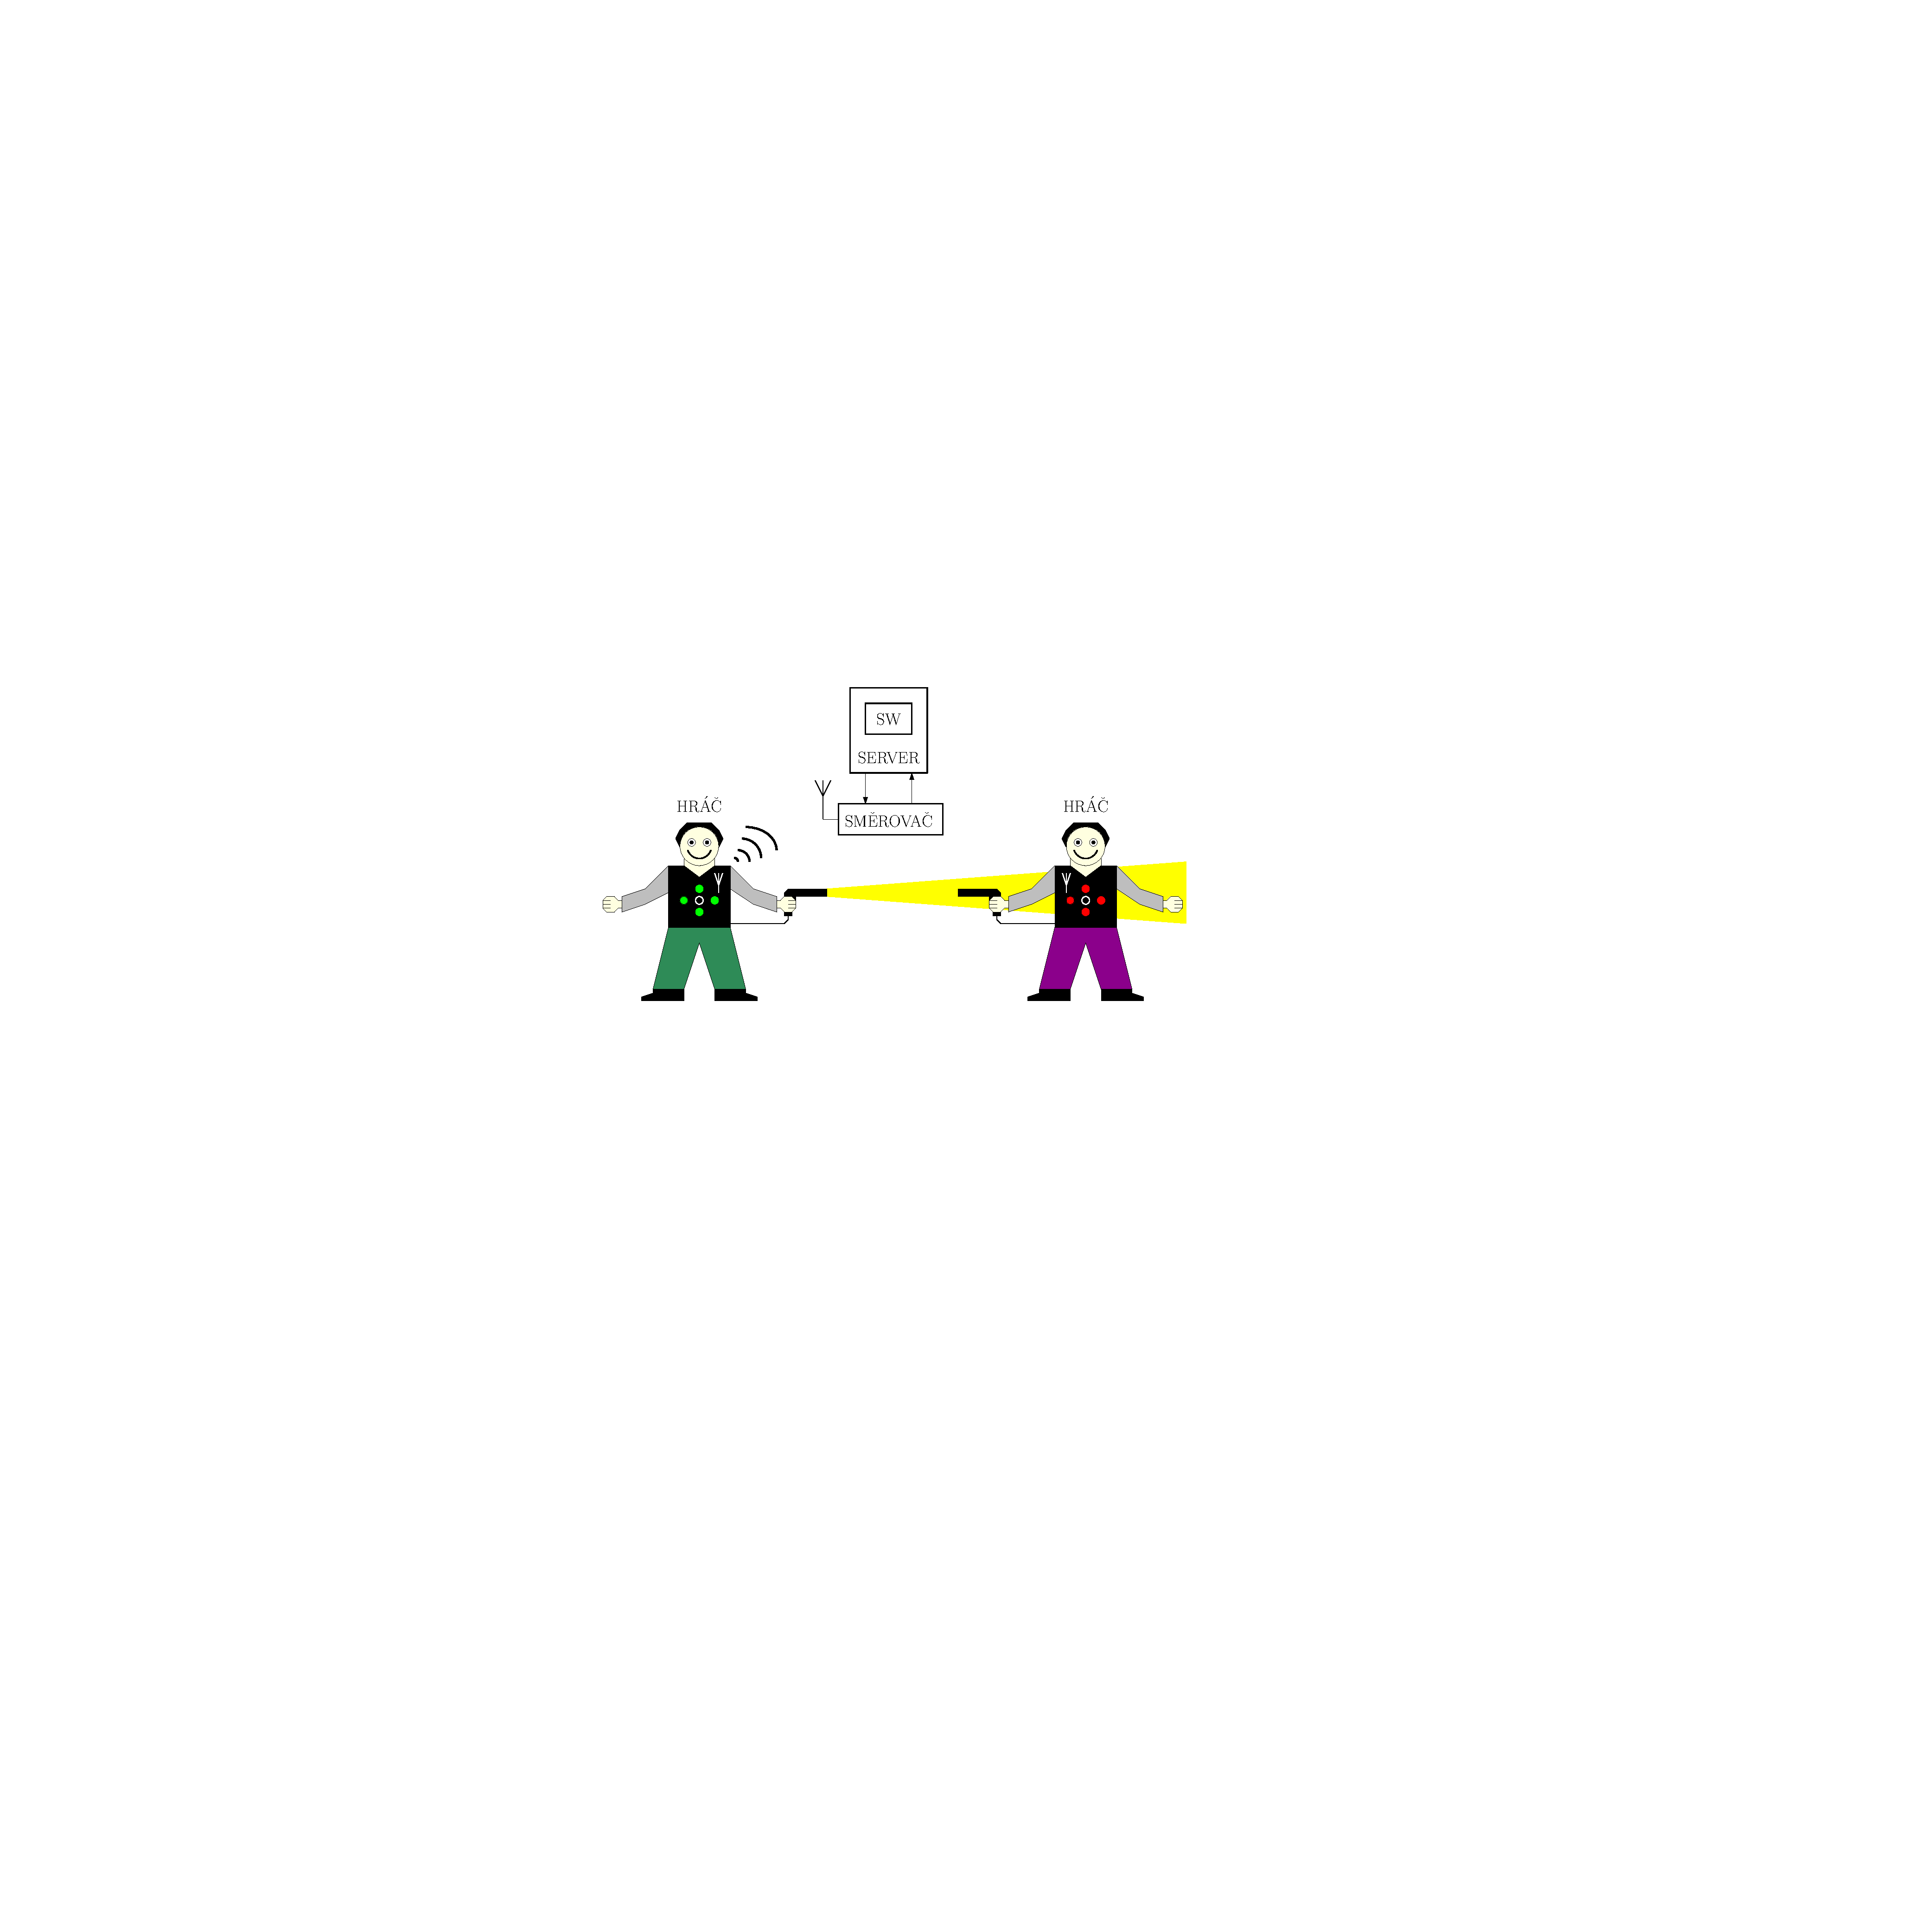
\includegraphics[width=\textwidth]{img/lgs}
    \end{center}
    \caption{Znázornění \zkratka{LG} systému}
\end{figure}

\subsection{Řídící počítač}
Řídící počítač má za úkol prostřednictvím routeru komunikovat s vestami, případně i dalšími zařízeními v síti. Hostuje řídící \zkratka{SW}, pomocí něhož operátor arény ovládá hru. Zajišťuje nakonfigurování vest. V průběhu hry stahuje z vest údaje a vyhodnocuje pořadí hráčů. Často bývá doplněn tiskárnou, díky níž po vyhodnocení hry vytiskne každému hráči tabulky s informacemi o odehrané hře doplněné individuálními statistikami.

\subsection{Router}
Zajišťuje směrování v bezdrátové \zkratka{LG} síti. Zprostředkovává tedy duplexní spojení mezi vestami a počítačem.

\subsection{Vesta}
Vesta je oděv, který nosí hráči \zkratka{LG}. Má dvě hlavní funkce, detekovat zásahy a komunikovat s řídícím počítačem. Další funkcí vesty je barevná identifikace hráčů pomocí \zkratka{RGB} \zkratka{LED}. Vesta může zajišťovat i zvukové efekty, či zobrazovat hráči jeho statistiky z aktuální hry. Vesta také komunikuje s hráčovou zbraní, vyhodnocuje jestli hráč může střílet. Někdy může být vesta nahrazena systémem tagů upevněných na oblečení, tato varianta ale není moc oblíbená, protože upevňování tagů je zdlouhavé, navíc během hry hrozí jejich odpadnutí.

\subsection{Zbraň}
Zbraň má jednoduchou úlohu, zajišťuje vysílání \zkratka{IR} paprsku, který při zásahu vesty zabije hráče (jde o zabití ve hře ne o skutečné usmrcení). Také může obsahovat \zkratka{IR} detektor, díky kterému může být detekováno poškození zbraně jejím zásahem. Kromě toho může být i zbraň vybavena signalizační \zkratka{RGB} pro identifikaci teamu, svítilnou nebo displayem.
